\chapter{Markov Decision Processes}
\label{ch_mdp}

At first, we look at Markov chains, a simpler type of
probabilistic processes which do not offer choices to be made.
Then we generalize to Markov Decision Processes.
After that, we introduce the problem of {\em verification} (checking if a
given MDP satisfies a given property), overview known solutions with
a focus on value iteration and Bounded
Real-Time Dynamic Programming which will be used in later chapters.

It is assumed the reader is familiar with basic notions of probability
theory, namely those of {\em probability space} and {\em probability measure}.
Function $f : X \to [0,1]$ is a {\em probability distribution} over
a countable set $X$ if $\sum_{x \in X} f(x) = 1$.
$\distribution{S}$ denotes the
set of probability distributions on a set $S$.
Usually the probability space $(\Omega, \mathcal{F}, P)$
is implicitly known and we use $P(E)$ to
denote the probability of an event $E$.
We refer the reader to
\parencite{probability} for a proper treatment of probability theory.

\section{Markov Chains}

Markov chain is a simpler formalism than
Markov decision process and provides a good first intuition about
probabilistic models. In a Markov chain, there are no decisions, only
probabilities of transition.

\begin{definition}
    Let $S$ be a finite set of states.
    A sequence of random variables $(X_i : S \to \{0,1\})^{\infty}_{i=0}$
    is called a {\em finite discrete-time time-homogeneous Markov chain},
    if the probability of moving to a state is given only by the
    current state, that is\footnote{The first condition ensures that
    only the last state of ``history'' is considered, the second that
    the length of the history does not matter either.}
    $P(X_{k+1} = s_{k+1} \mid X_k = s_k) =
    P(X_{k+1} = s_{k+1} \mid X_k = s_k, X_{k-1} = s_{k-1}, \ldots, X_{1} = s_{1})$
    for every $s_k \in S$,
    if the conditional probabilities are defined,
    and
    $P(X_{k+1} = s_{k+1} \mid X_k = s_k)
    = P(X_{k} = s_{k} \mid X_{k-1} = s_{k-1})$.
\end{definition}

In many applications it is natural to have an initial state
$s$ ($X_1 = s$) and a chain can
then be drawn as a graph with probabilistic transitions. Note
that the weights of the outgoing edges from a node sum to one, as the
transition probabilities form a distribution on the set of states (for
simplicity we do not draw the transitions with zero probability).

\begin{example}
    \label{ex_mc}
    In this example $s_0$ is the initial state,
    $P(X_2 = s_1 \mid X_1 = s_0) = 0.5$,
    $P(X_2 = s_2 \mid X_1 = s_0) = 0.25$,
    $P(X_2 = s_0 \mid X_1 = s_0) = 0.25$,
    $P(X_{i+1} = s_1 \mid X_{i} = s_1) = 1$,
    $P(X_{i+1} = s_2 \mid X_{i} = s_2) = 1$,
    for all $i \in \mathbb{N}$.

\hfill \break
\centering
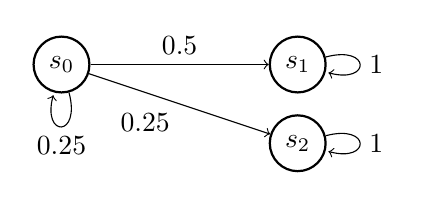
\begin{tikzpicture}
    \tikzstyle{state}=[thick,draw=black,circle]
    \tikzstyle{decision}=[draw,shape=circle,fill=black]

    %\node[state] at (0,0) (s0) {$s_0$};
    %\node[state] at (2,0) (s0b) {};
    %\node[state] at (4,0) (s1) {$s_1$};
    %\node[state] at (4,-1) (s2) {$s_2$};

    %\draw (s0) edge [bend left, ->] node [midway, above] {} (s0b);
    %\draw[->] (s0b) -- (s1) node [midway, above] {0.5};
    %\draw (s0b) edge [bend left, ->] node [midway, below] {0.25} (s0);
    %\draw[->] (s0b) -- (s2) node [midway, below left] {0.25};
    \node[state] at (0,0) (s0) {$s_0$};
    \node[state] at (3,0) (s1) {$s_1$};
    \node[state] at (3,-1) (s2) {$s_2$};

    \draw[->] (s0) -- (s1) node [midway, above] {0.5};
    \draw (s0) edge [->, loop below] node [midway, below] {0.25} (s0);
    \draw[->] (s0) -- (s2) node [midway, below left] {0.25};

    \draw (s1) edge [->, loop right] node [midway, right] {1} (s1);
    \draw (s2) edge [->, loop right] node [midway, right] {1} (s2);
\end{tikzpicture}
\end{example}

\begin{example} The Drunkard's Walk is a well-known example of a Markov
    chain. One can imagine a drunk person starting in the middle of a road
    (state $s_0$) and then moving left or right at random. How many times
    will the drunk visit the middle of the road? How many steps will it
    take the drunk on average to reach a ditch ($s_{-2}, s_2$)?

\hfill \break
\centering
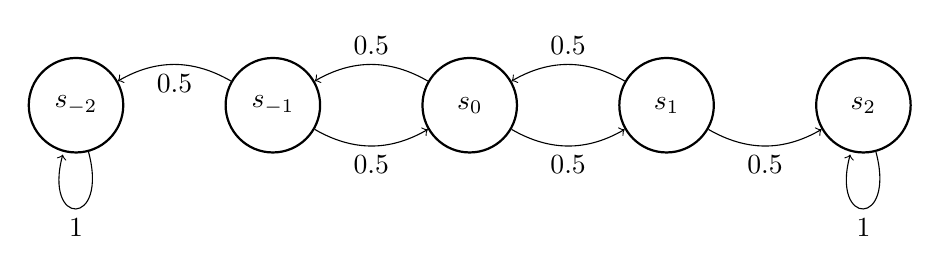
\begin{tikzpicture}
    \tikzstyle{state}=[thick,draw=black,circle, minimum size=1.2cm]
    \tikzstyle{decision}=[draw,shape=circle,fill=black]

    \node[state] at (-5,0) (sm2) {$s_{-2}$};
    \node[state] at (-2.5,0) (sm1) {$s_{-1}$};
    \node[state] at (0,0) (s0) {$s_0$};
    \node[state] at (2.5,0) (s1) {$s_1$};
    \node[state] at (5,0) (s2) {$s_2$};

    \draw (sm2) edge [->, loop below] node [midway, below] {1} (sm2);
    \draw (sm1) edge [->, bend right] node [midway, below] {0.5} (sm2);

    \draw (s0) edge [->, bend right] node [midway, above] {0.5} (sm1);
    \draw (sm1) edge [->, bend right] node [midway, below] {0.5} (s0);

    \draw (s0) edge [->, bend right] node [midway, below] {0.5} (s1);
    \draw (s1) edge [->, bend right] node [midway, above] {0.5} (s0);

    \draw (s1) edge [->, bend right] node [midway, below] {0.5} (s2);
    \draw (s2) edge [->, loop below] node [midway, below] {1} (s2);
\end{tikzpicture}
\end{example}

\section{Markov Decision Processes}

Markov decision processes are similar to Markov chains, except now a
controller interacting with the process can in each state pick an action
and the next state is chosen according to a distribution on states
corresponding to this action.

\begin{definition}
A {\em Markov Decision Process} is a tuple $(S, s_0, A, E, \Delta)$, where
$S$ is a finite set of states,
$s_0 \in S$ is the initial state,
$A$ is a finite set of actions,
$E : S \to \powerset{A}$ gives the set of enabled actions in a state,
and $\Delta : S \times A \to \distribution{S}$ is a partial transition
function which assigns a probability distribution on states to an action
and a state.

It is assumed without loss of generality that for all $s \neq s'$ it
holds that $E(s) \cap E(s') = \emptyset$. If this did not hold the
actions could just be renamed.
\end{definition}

\begin{example}
    \label{ex_mdp}
    The MDP $(\{s_0, s_1, s_2\}, s_0, \{a, b\}, E, \Delta)$,
    where
    $E(s_0) =$ \linebreak $\{a,b\}$,
    $E(s_1) \{c\}, E(s_2) = \{d\}$,
    and $\Delta(s_0, a) = \{(s_1, 1)\}$,
    $\Delta(s_0, b) = \{(s_1, 0.5),$ $(s_2,0.25), (s_0,0.25)\}$,
    $\Delta(s_1,c) = \{(s_1,1)\},
    \Delta(s_2,d) = $ \linebreak $ \{(s_2,1)\}$
    is depicted below.
    The edges labeled with letters denote the available actions
    and lead to smaller black dots, which mark the point of random
    choice of the successor state. With actions $c,d$ the black dots are
    omitted and the transition probability 1 is understood implicitly.

    The controller making decisions should choose action $a$ if
    they want to get to $s_1$, or (possibly repeatedly) choose $b$ if
    they want to get to $s_2$ (the achievement of this goal is not
    guaranteed).

\hfill \break
\centering
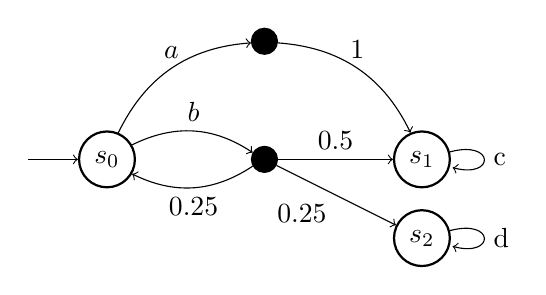
\begin{tikzpicture}
    \tikzstyle{state}=[thick,draw=black,circle]
    \tikzstyle{transition}=[draw,shape=circle,fill=black]

    \node[state] at (0,0) (s0) {$s_0$};
    \node[transition] at (2,1.5) (s0a) {};
    \node[transition] at (2,0) (s0b) {};
    \node[state] at (4,0) (s1) {$s_1$};
    \node[state] at (4,-1) (s2) {$s_2$};

    \draw[<-] (s0) -- node[above] {} ++(-1cm,0);

    \draw (s0) edge [bend left, ->] node [midway, above] {$a$} (s0a);
    \draw (s0a) edge [bend left, ->] node [midway, above] {$1$} (s1);
    \draw (s0) edge [bend left, ->] node [midway, above] {$b$} (s0b);
    \draw[->] (s0b) -- (s1) node [midway, above] {0.5};
    \draw (s0b) edge [bend left, ->] node [midway, below] {0.25} (s0);
    \draw[->] (s0b) -- (s2) node [midway, below left] {0.25};

    \draw (s1) edge [->, loop right] node [midway, right] {c} (s1);
    \draw (s2) edge [->, loop right] node [midway, right] {d} (s2);
\end{tikzpicture}

\end{example}

A standard use of Markov decision processes has been in areas where it
is useful to operate with rewards.

\begin{definition}
If $(S, s_0, A, E, \Delta)$ is a Markov decision process,
%$a \in A, s, s' \in S$, $a \in E(s)$, $\Delta(s,a)(s') > 0$,
and \linebreak $R : S \times A \times S \to \mathbb{R}$ is a function,
then $(S, s_0, A,E,\Delta,R)$ is a {\em Markov decision process with rewards}.
\end{definition}


\begin{definition}[Path]
    An {\em infinite path} is
    a sequence $\omega = s_0 a_0 s_1 a_1
    \ldots$ such that $a_i \in E(s_i)$ for all $i \in \mathbb{N}$.
    The set of all infinite paths of is denoted $IPaths$.

    A {\em finite path} is a prefix of an infinite path such that it
    ends with a state. The last state for a finite path $\rho$ is
    denoted $\last(\rho)$. The set of all finite paths is denoted
    $FPaths$.
\end{definition}

When following a path one wants to avoid getting stuck in
an infinitely repeated cycle of states and actions. The parts of MDP
where this happens are called end components.
An example end component is shown in \autoref{fig:non-triv-ec}.

\begin{definition}[End component]
Let $\mathcal{M} = (S, s_0, A, E, \Delta)$ be an MDP,
let $S' \subseteq S$ and $A' \subseteq \bigcup_{s' \in S'} E(s')$.
The pair $(S', A')$ is an {\em end component},
if for every $s \in S', s' \in S, a \in A'$ it holds that
$$\Delta(s,a)(s') > 0 \implies s' \in S'$$
and there is a path between every two $s, s' \in S'$
using only actions $A'$.

An end component is {\em maximal} if it is maximal with respect to
the point-wise ordering of subsets.
\end{definition}

\begin{figure}[ht]
\begin{center}
\begin{tikzpicture}
    \tikzstyle{state}=[thick,draw=black,circle]
    \tikzstyle{transition}=[draw,shape=circle,fill=black]

    \draw[<-] (s0) -- node[above] {} ++(-1cm,0);

    \node[state] at (0,0) (s0) {$s_0$};
    \node[state] at (2,0) (s1) {$s_1$};
    \node[state] at (4,0) (s2) {$s_2$};

    \draw (s0) edge [bend left, ->] node [midway, above] {$a$} (s1);
    \draw (s1) edge [bend left, ->] node [midway, below] {$b$} (s0);
    \draw (s1) edge [->] node [midway, above] {$c$} (s2);

    \draw (s2) edge [->, loop right] node [midway, right] {d} (s2);
\end{tikzpicture}
\end{center}
\caption{An MDP with a non-trivial end component.}
\label{fig:non-triv-ec}
\end{figure}

The following definition introduces what is commonly called strategy,
policy, scheduler, controller or adversary. It is the decision maker in
the MDP which looks at the path traversed so far and assigns each action
$a$ in the last (current) state the probability of $a$ being chosen.

\begin{definition}[Strategy]
    Let $\mathcal{M} = (S,A,E,\Delta)$ be a Markov decision process
    and $\rho \in FPaths$.
    A {\em strategy} is a function
    $\sigma : FPath \to Dist(A)$
    such that\footnote{
The condition ensures that only actions which can
be chosen have non-zero probability assigned by the strategy.}
    $\sigma(\rho)(a) > 0 \implies a \in E(\last(\rho))$.

    A strategy $\sigma$ is {\em memoryless} if $\sigma(\rho)$ depends
    only on $\last(\rho)$. A strategy $\sigma$ is {\em deterministic}
    if $\sigma(\rho)(a) = 1$ for some $a \in E(\last(\rho))$.
\end{definition}

What happens once the strategy is fixed? The MDP becomes a Markov chain.
This can be seen in the examples, e.g. if the strategy is to always
choose $b$, the MDP from \autoref{ex_mdp} becomes the MC from
\autoref{ex_mc}.
Importantly when a strategy is fixed there is a probability
measure\footnote{While this may be intuitive it is not a trivial
statement, see Theorem 2.4 in \parencite{denumerable_mc} for a formal
treatment.} denoted $P^\sigma_{\mathcal{M},s}$ over the set of
$IPaths$ with an initial state $s$, which assigns to a set of paths the
probability they will be traversed.

%For very small MDPs this gives the first algorithm for evaluating
%their properties: for every strategy reduce the MDP to a Markov chain
%and evaluate the property using known Markov chain algorithms, then
%aggregate the results\footnote{The idea of this naive method can be
%significantly improved and instead of exploring a vast amount of
%strategies only a small portion of reasonably good strategies is
%explored \parencite{smc}.}.

\noindent {\bf Completeness of information about an MDP.}
One can distinguish between various levels of knowledge about an MDP,
usually, depending on the source of the model.
Complete information corresponds to knowing every part of the
definition of an MDP, as opposed to limited information where the MDP
can only be used as a black box from which can information be extracted
by sampling.
%For example $\Delta$ might
%not be known.
%he information about $\Delta$ may not be available (but
%reachability can still be effectively solved \parencite{atva14}).
This thesis is concerned only with MDPs with complete information.


\section{Verification}

{\em Formal verification} is the act of proving that a given system satisfies
a given property. {\em Model
checking} is an approach to formal verification which uses a model of
the system to verify the property.

In our case, the systems are modeled as Markov decision processes and
the properties are concerned about the maximum probability of reaching a
state.

To simplify notation, in this section we often refer to a fixed MDP $\mathcal{M} =
(S,s_0,A,E,\Delta)$, and a set of target states $F$.

\noindent \textbf{Reachability probability.}
Let $\lozenge F$ be the set of all infinite paths that reach a state in $F$.
In this thesis we are concerned with maximising the reachability
probability $P^\sigma_{\mathcal{M},s_0}(\lozenge F)$ over the set of all
strategies $\sigma$.
We define the {\em value function} $V(s) = \sup_{\sigma}
P^\sigma_{\mathcal{M},s}(\lozenge F)$ for every state $s \in S$.

Importantly there is always a memoryless, deterministic strategy maximising the
reachability probability. This was proven by Puterman \parencite{puterman}
for reward maximization and the proof can be used with a simple
reduction for the case of verification \parencite{verification_complexity}.
For any MDP create an MDP with rewards, such that the reward function
is zero everywhere, except when entering a target state it gives reward 1
and then transitions into a new sink state (with reward 0).

In this section, we describe value iteration,
which is a standard algorithm for computing the maximum probability of
reaching a state in F. In the next section, a more involved algorithm
called BRTDP is described.

One approach not explained here is so-called {\em strategy iteration}
which starts with an arbitrary strategy and gradually improves it as
long as a change to the strategy is beneficial. Strategy iteration has
a clear stopping criterion as opposed to value iteration, however, in
practice, it does not perform better \parencite{forejt}.

Another approach we do not explain is formulating the problem as a system
linear equations and solving it. The solution is precise and has
guaranteed correctness, but the computation quickly becomes expensive as
the model grows in size.  See \parencite{forejt} for a description of
this method.

\subsection*{Value Iteration}

Value iteration (in its variation for computing expected maximum rewards) is a
dynamic programming algorithm which was first described by Richard
Bellman\footnote{Known for introducing the term dynamic programming.}
\parencite{bellman} in 1957. We present its variation for computing the maximum
reachability probability.

Before showing the algorithm, we first note that it will need to
process all states. However, the values in some states are quite easy to
compute and a preprocessing will allow for reduction of the
state space.
These easy states are in set $Z \subseteq S$
of {\em zero states} or set $F' \subseteq S$ of {\em extended target states}.
States $z \in Z$ are such that $P^\sigma_{\mathcal{M},z}(\lozenge F) = 0$ holds,
and states $f \in F'$ are such that $P^\sigma_{\mathcal{M},f}(\lozenge F) = 1$
holds, both for any strategy $\sigma$.
Their computation is rather straightforward \parencite{forejt} (Section
4.1). Note that $F \subseteq F'$.

The main idea of value iteration is materialized in the following
recurrence relation for newly introduced variables $x_s^n, s \in S, n
\in \mathbb{N}$.
\[
x_s^n =
\begin{cases}
    1 & \text{if }s \in F' \\
    0 & \text{if }s \in Z \lor (s \not \in F' \land n = 0) \\
    \max\limits_{a \in E(s)} \sum\limits_{s' \in S} \Delta(s,a)(s') \cdot x_{s'}^{n-1}
    & \text{otherwise} % \text{if }s \in S \setminus (F \cup Z)
\end{cases}
\]
By computing $x^n$ for $n = 1,2,\ldots$ we gain increasingly precise
estimate of the actual maximum reachability probability,
formally $\lim_{n \to \infty} x^n_s = P_{\mathcal{M},s}(\lozenge F)$.
We refer to a proof of this statement in \parencite{puterman} with the
same reduction as in the case of existence of memoryless optimal
strategy.

This recurrence relation is now turned into a dynamic programming
algorithm as shown in \autoref{vi}. Instead of iterating $n$ times, the
algorithm proceeds with its computations while the convergence is not
slow (the threshold is given by some $\epsilon$).

\begin{algorithm}
\caption{Value Iteration}
\label{vi}
\begin{algorithmic}
    \State $\forall s \in S,\; s \gets 1$ if $x \in F$ else $0$
    \Do
        \ForEach{$s \in S \setminus (F \cup Z)$}
            \State $x_s \coloneqq
            \max_{a \in E(s)} \sum_{s' \in S} \Delta(s,a)(s') \cdot x_{s'}$
        \EndFor
    \doWhile{the change of $x_s$ for any $s$ is greater than $\epsilon$}
\end{algorithmic}
\end{algorithm}

Value iteration is an easy method for computing the reachability
probability of a given MDP.  However, we only have a proof of convergence
and not a useful stopping criterion.  Furthermore, it is doing extra work
on models where only a small part needs to be explored to find a good
strategy as it has to compute its results for all the states.

The solution to the first issue is the {\em interval iteration}
algorithm \parencite{interval_iteration}, an algorithm in parts similar
to value iteration but which maintains lower and upper bounds of the
sought probability. The algorithm has a well-defined stopping criterion
and a bound on the running time.  We will explore solutions to the
second issue later with heuristic methods.

% http://www.sciencedirect.com/science/article/pii/S0304397516307095
% http://pageperso.lif.univ-mrs.fr/~benjamin.monmege/talks/MoVe2015.pdf

\section{Bounded Real-Time Dynamic Programming}
\label{sec:brtdp}

When only a portion of an MDP needs to be searched to find the right
strategy there is an opportunity to employ algorithms which avoid
searching the whole state space. Bounded Real-Time Dynamic Programming
(BRTDP) is such an algorithm. Originally developed for
the objective of finding the best-profit strategy
\parencite{profit_brtdp} the algorithm was adapted to the problem of
verification \parencite{atva14}.

As in the previous section, we refer to a fixed MDP $\mathcal{M} =$
\linebreak $(S,s_0,A,E,\Delta)$, and a set of target states
$F$. Further we fix $\epsilon$, an argument of the algorithm which sets
the required precision (maximum allowed distance of the result of the
algorithm from the correct value).

Recall we have a unary value function defined
and for use in the algorithm let us define the binary {\em value function}
$V : S \times A \to [0,1]$ for all $s \in S$ and $a \in E(s)$ as follows
\[
    V(s,a) \coloneqq \sum_{s' \in S} \Delta(s,a)(s')V(s')
\]
This serves to represent the value in $s$ after taking action $a$.
BRTDP is learning $V$ by monotonically tightening its lower and upper
bounds $L, U : S \times A \to [0,1]$ during simulated runs of
$\mathcal{M}$ from the given initial state.
When $\max_{a \in E(s_0)} U(s_0, a) - \max_{a \in E(s_0)} L(s_0, a) < \epsilon$
the algorithm terminates.

We start with an important assumption, that
that $\mathcal{M}$ does not contain any end component
besides two trivial end components, one containing only the target state
1 with $F = \{1\}$, the other only the state 0 with $V(0) = 0$.

With this assumption BRTDP can be implemented as \autoref{alg:brtdp},
alternating between simulation and update phases until it has
sufficiently good knowledge about $V(s_0)$. In the simulation phase the,
algorithm samples a finite path from the initial state to one of states
$\{1, 0\}$, each time using an action maximising the upper bound.
In the update phase, the algorithm traverses the path backwards and
performs the Bellman update (known from value iteration),
using the best-known bounds, i.e.
$U(s) = \max_{a \in E(s)} U(s, a)$
and
$L(s) = \max_{a \in E(s)} L(s, a)$.
With the assumption of no non-trivial BRTDP converges almost surely to the correct value \parencite{atva14},
that is
the actual probability almost always lies between $L(s_0), U(s_0)$,
and the bounds converge such that they are at most $\epsilon$ (for a
given $\epsilon$) far from each other.


\begin{algorithm}
\caption{BRTDP for MDPs without end components}
\label{alg:brtdp}
\begin{algorithmic}
\State $U(s,a) \gets 1, L(s,a) \gets 1 \; \forall s \in S, a \in E(s)$
\State $U(0,a) \gets 0, L(1,a) \gets 1 \; \forall a \in A$
\State $\omega \gets s_0$
\While{$U(s_0) - L(s_0) < \epsilon$ }
    % simulation
    \State \# Simulation Phase
    \While{$last(\omega) \not \in \{0,1\}$}
        \State $a \gets$ sample uniformly from
           $\argmax\limits_{a \in E(last(\omega))}
            U(last(\omega), a)$
        \State $s \gets$\footnote{The implementation of this line may
            vary, see Subsection ``Variants of BRTDP''}
            sample according to $\Delta(last(\omega), a)$
        \State $\omega \gets \omega \; a \; s$
    \EndWhile

    % update
    \State \# Update Phase
    \While{$\omega$ is not empty}
        \State $pop(\omega)$
        \State $a \gets pop(\omega)$
        \State $s \gets last(\omega)$
        \State $U(s,a) \coloneqq \sum_{s' \in S} \Delta(s,a)(s') U(s')$
        \State $L(s,a)\, \coloneqq \sum_{s' \in S} \Delta(s,a)(s') L(s')$
    \EndWhile
\EndWhile
\State \Return $(U(s_0), L(s_0))$
\end{algorithmic}
\end{algorithm}

\subsection*{BRTDP for MDPs with End Components}
\autoref{alg:brtdp} is not guaranteed to converge
when the MDP contains non-trivial end components.

\begin{example}
    Below is an MDP with an end component
    $(\{s_0, s_1\}, \{a,c\})$, and let $F = \{s_2\}$.
    When BRTDP updates state $s_0$ or $s_1$ there is always a state (the
    other one in the EC) which has upper bound 1. This way the upper
    bound remains 1 after every iteration, even though the lower bound
    is correctly $0.5$. The algorithm does not converge for $\epsilon <
    0.5$.

\begin{center}
\begin{tikzpicture}
    \tikzstyle{state}=[thick,draw=black,circle]
    \tikzstyle{transition}=[draw,shape=circle,fill=black]

    \draw[<-] (s0) -- node[above] {} ++(-1cm,0);

    \node[state] at (0,0) (s0) {$s_0$};
    \node[state] at (2,0) (s1) {$s_1$};
    \node[transition] at (4,0) (s0b) {};
    \node[state] at (6, 0.7) (s2) {$s_2$};
    \node[state] at (6,-0.7) (s3) {$s_3$};

    \draw (s0) edge [bend left, ->] node [midway, above] {$a$} (s1);
    \draw (s1) edge [bend left, ->] node [midway, below] {$b$} (s0);
    \draw (s1) edge [->] node [midway, above] {$c$} (s0b);

    \draw[->] (s0b) -- (s2) node [midway, above] {0.5};
    \draw[->] (s0b) -- (s3) node [midway, below] {0.5};

    \draw (s2) edge [->, loop right] node [midway, right] {d} (s2);
    \draw (s3) edge [->, loop right] node [midway, right] {e} (s3);
\end{tikzpicture}
\end{center}
\end{example}

Fortunately, there is an on-the-fly method\footnote{The knowledge we have
about the MDP during computation suffices -- knowing the whole MDP is
not necessary.}
for resolving the problem in BRTDP
\parencite{atva14}, which we present to an extent important for our
future use of BRTDP.

During the simulation phase, the algorithm periodically (every $k_i$
steps) creates an auxiliary MDP based on the states visited so far and
their neighbours. The algorithm then identifies maximal ECs in this auxiliary
MDP.

If an end component is found it is collapsed, i.e. the states are merged into a
single state and functions $E, \Delta$ are naturally transformed to work
the same way in the modified MDP.

Finally, the merged state has its $U, L$ updated for every action in the
end component. If there was a target state in the end component then the
merged state is marked as a target state. If there was no target state and
there is no outgoing action from the merged state then it is marked as a
zero state.

\subsection*{Variants of BRTDP}
When BRTDP is in state $s$ and it has chosen action $a$,
the choice of the next state does not necessarily have to be done by
sampling the transition distribution $\Delta(s,a)$ (we call this variant
HIGH-PROB) but can be instead chosen with probability
$\Delta(s,a)(s') \cdot (U(s') - L(s'))$, we call this variant MAX-DIFF.
One can think of other variants, for example round-robin choice.

\begin{example}
\label{brtdp_adversary}
We conclude with an example MDP, which is hard for most variants of
BRTDP when the target is the final state.
For example the HIGH-PROB variant has probability $0.99$ of returning to
the initial state from every state until reaching the final state.

\begin{center}
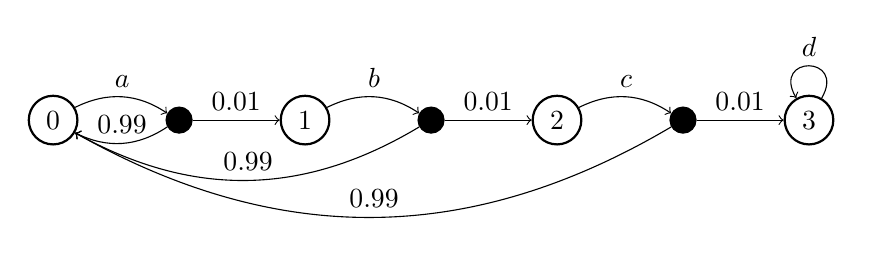
\begin{tikzpicture}
    \tikzstyle{state}=[thick,draw=black,circle]
    \tikzstyle{transition}=[draw,shape=circle,fill=black]
    \tikzstyle{loop}=[looseness=5, in=120, out=60]

    \node[state] at (0,0) (s0) {0};
    \node[transition] at (1.6,0) (s0b) {};
    \node[state] at (3.2,0) (s1) {1};
    \node[transition] at (4.8,0) (s1b) {};
    \node[state] at (6.4,0) (s2) {2};
    \node[transition] at (8,0) (s2b) {};
    \node[state] at (9.6,0) (s3) {3};

    \draw (s0) edge [bend left, ->] node [midway, above] {$a$} (s0b);
    \draw[->] (s0b) -- (s1) node [midway, above] {0.01};
    \draw (s0b) edge [bend left, ->] node [midway, above] {0.99} (s0);

    \draw (s1) edge [bend left, ->] node [midway, above] {$b$} (s1b);
    \draw[->] (s1b) -- (s2) node [midway, above] {0.01};
    \draw (s1b) edge [bend left, ->] node [midway, above] {0.99} (s0);

    \draw (s2) edge [bend left, ->] node [midway, above] {$c$} (s2b);
    \draw[->] (s2b) -- (s3) node [midway, above] {0.01};
    \draw (s2b) edge [bend left, ->] node [midway, above] {0.99} (s0);

    \draw (s3) edge [loop,->] node [above] {$d$} (s3);
\end{tikzpicture}
\end{center}
\end{example}
